% !TEX root = ../ITGO.tex

\subsection*{Three-bar truss design problem}

The three-bar truss design problem \citep{TB} consists in minimizing the volume of a statically loaded three-bar truss. There are two continuous design variables and three nonlinear inequality constraints, based on the stress on each of the truss members ($\sigma$), with $f(\bm{x}^*) = 263.895843$. Figure \ref{fig:TB} shows the schematic view of the problem.

\begin{figure}[h]
    \begin{center}
    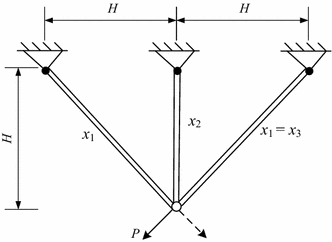
\includegraphics[scale=0.5]{Imgs/TB.png}
    \end{center}
    \captionsetup{justification=centering}
    \caption{Schematic view of the three-bar truss design problem.}\label{fig:TB}
\end{figure}

\prob{Appendix/Problems/TB}